\section{Methodology}

Initially, the current and previous identity management systems have been studied. The first step is to 
digitalize the current identities and make it reliable for identity owners. After a thorough literature 
review, an approach is found: self-sovereign identity. And the next objective is to implement it in the 
real world. and the proposed solution is as follows.

\begin{figure}[H]
    \centering
    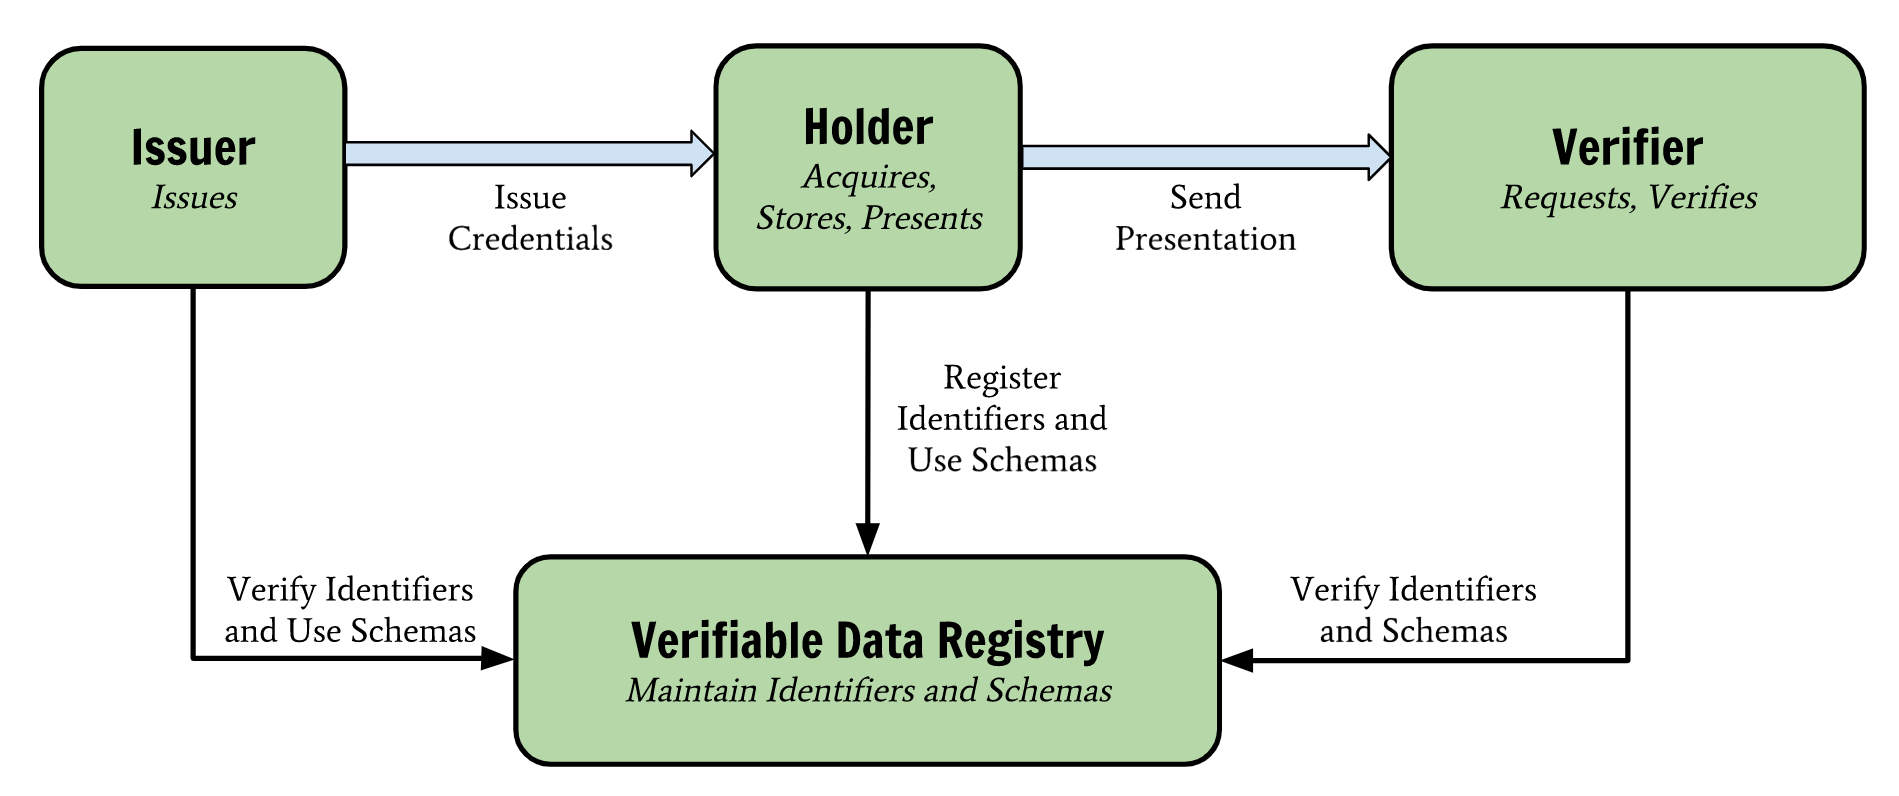
\includegraphics[scale=0.4]{13.png}
    \caption{methodology architecture}
    \label{fig:threshold}
  \end{figure}

  There are 3 main roles in this proposed design.
\begin{enumerate}
    \item Issuer
    \item Holder
    \item Verifier
\end{enumerate}

\begin{itemize}
    \item The holder is the one who wants to verify documents through the system when the holder needs to get credentials for his identity(a legal document or a claim), the issuer should issue the credentials.
    \item Before issuing the credentials, the issuer needs to contact the government or a trust anchor in the system, to get the schema of the particular identity.
    \item Then issuer can issue the credentials to the user(holder) and send verify the identifiers using the trust anchor.
    \item The holder stores the credentials for his particular identity in his wallet.whenever the holder needs to use the credential on a different organization holder sends the credentials.
    \item Verifier verifies the credentials using the system.
\end{itemize}

In order to implement this design, blockchain is the most suited technology because blockchain holds the properties of self-sovereign identity and make the system more reliable in between users.
  

